\def\MyCourse{データサイエンスコース}
\def\MySubject{R入門}
\def\MySemester{春学期}

\newcommand{\R}{\textbf{R}}
\newcommand{\RStudio}{\textbf{RStudio}}
\newcommand{\Excel}{\textbf{Excel}}
\newcommand{\cs}[1]{\textcolor{blue}{\texttt{#1}}} % Console prompt >


\subsection{描画用データ作成}

\myffr

\mybfr{手順}
描画用データとして,平均,標準偏差が異なる3種類の正規乱数(N=100)を作成する.
また,表示用の色をそれぞれ作成する.
\mybto

\begin{minipage}{0.45\hsize}

\lstinputlisting[firstline=1,lastline=21]{graph.r}

\end{minipage}
\hspace{3mm}
\begin{minipage}{0.5\hsize}
\mybfr{演習}
左のソースコードを「graph.r」として保存してください.\\
色彩名表示colors()でどのような色があるか確認してください.
%「R」,「色見本」,「colors」などのキーワードで,インターネットでどのような色見本があるか検索してください.
\mybto
\mycheck{\tiny 色彩名 -> RGB変換: col2rgb('色彩名')}\\
\mycheck{\tiny 色彩名関数: rainbow(n), heat.colors(n), grey(1:11/12),\\\hfill terrain.colors(n), topo.colors(n), cm.colors(n)}\\
\mycheck{\tiny cf. \href{https://oku.edu.mie-u.ac.jp/~okumura/stat/colors.html}{奥村研究室,「統計グラフの色」}}
\end{minipage}

\end{frame}

\subsection{散布図}

\myffr

\begin{minipage}{0.45\hsize}
\tiny
\vspace{-3mm}
\lstinputlisting[language=R, firstline=3,lastline=21]{050-scatter.r}

\mybfr{演習}
グラフィックオプションは次のようなものがあります.\\
値を変更してグラフを変化させてみてください.\\ \relax
type=\{p, l, b, o, s, h, n\}, pch=0--25, lty=0--6
\mybto

\end{minipage}
\hspace{3mm}
\begin{minipage}{0.45\hsize}
\begin{figure}[t]
  \centering
  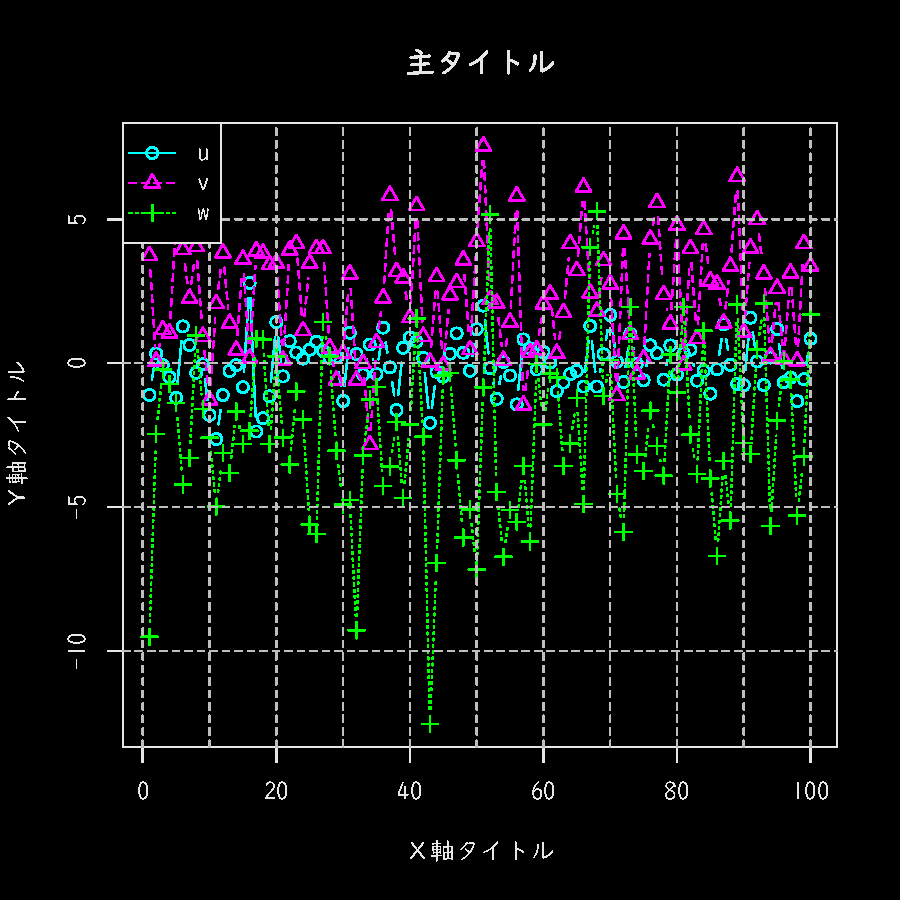
\includegraphics[width=\hsize]{fig/scatter}
  \caption{散布図描画例}
  \label{fig:scatter}
\end{figure}
\vspace{-5mm}

\mycheck{\tiny{type: plot \textbf{type}, col: plot \textbf{col}or, bg: \textbf{b}ack\textbf{g}round color}}\\
\mycheck{\tiny{pch: \textbf{p}oint \textbf{ch}aracter, lty: \textbf{l}ine \textbf{ty}pe, lwd: \textbf{l}ine \textbf{w}i\textbf{d}th}}\\
\mycheck{\tiny{h: \textbf{h}orizontal line, v: \textbf{v}ertical line}}\\

\end{minipage}

\end{frame}

\subsection{ヒストグラム}

\myffr

\begin{minipage}{0.45\hsize}
\tiny
\vspace{-3mm}
\lstinputlisting[language=R, firstline=3,lastline=26]{050-hist.r}

\end{minipage}
\begin{minipage}{0.45\hsize}
\begin{figure}[t]
  \centering
  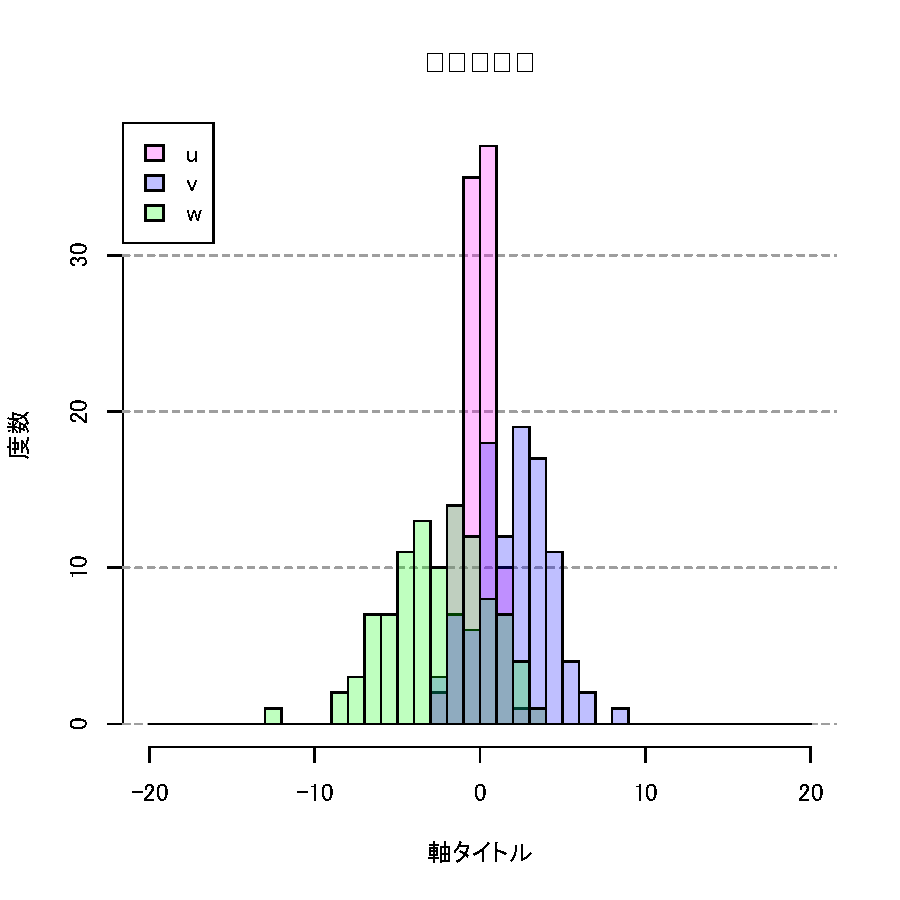
\includegraphics[width=\hsize]{fig/hist}
  \caption{ヒストグラム描画例}
  \label{fig:hist}
\end{figure}
\vspace{-5mm}
\mycheck{\tiny{add = T オプションで重ね書きができる}}\\
\mycheck{\tiny{rgb(red = 0, blue = 1, green = 0, alpha = .5)\\
               \hfill でRGB値を出力できる(alpha: 透明度)}}\\

\end{minipage}

\end{frame}

\subsection{回帰モデルグラフ}

\myffr

\begin{minipage}{0.50\hsize}
\tiny
\vspace{-3mm}
\lstinputlisting[language=R, firstline=3,lastline=28]{061-lm-plot.r}
\vspace{-4mm}
\normalsize
\end{minipage}
\begin{minipage}{0.45\hsize}

\begin{figure}[t]
  \centering
  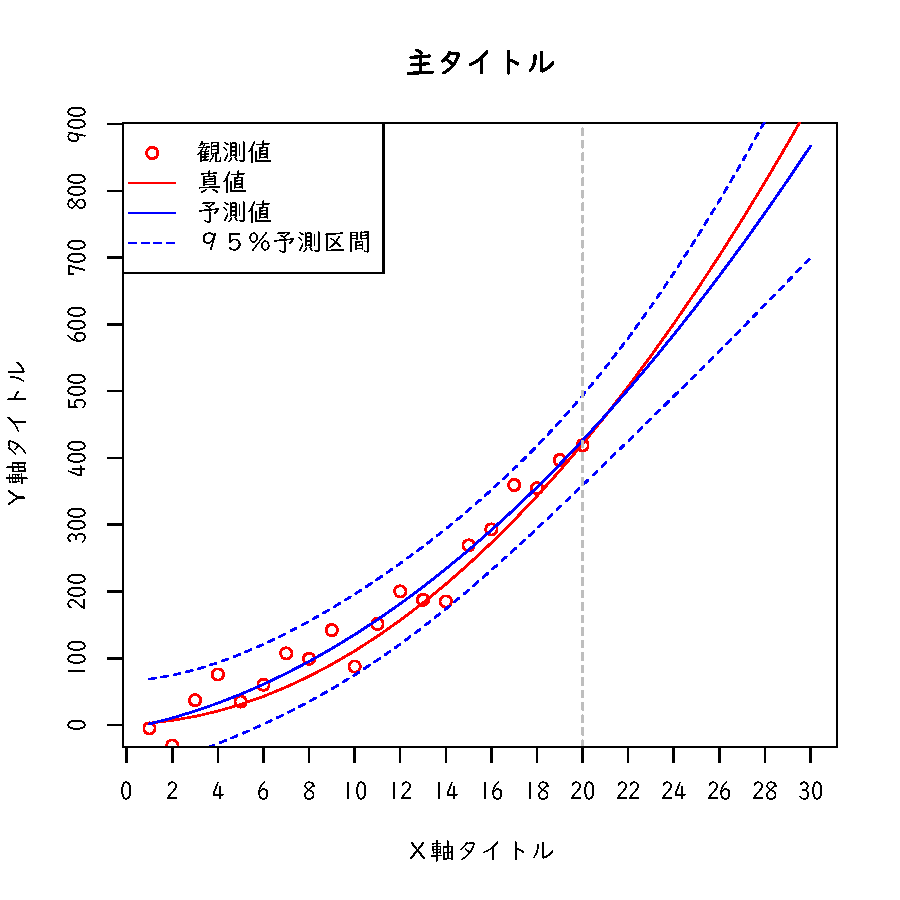
\includegraphics[width=\hsize]{fig/lm}
  \caption{回帰モデルグラフ描画例}
  \label{fig:lm50}
\end{figure}
\vspace{-8mm}
\mycheck{描画関数\tiny{matpoints: 点,matlines: 線,abline: 縦横線,axis: 軸,legend: 凡例}}\\
\mycheck{描画オプション\tiny{col: 色,pch: 点種,lty: 線種,v:縦線,h:横線}}

\end{minipage}

\end{frame}

\end{document}

